
\begin{itemize}
\item What is ECDAR
\item Purpose
\item Technologies
\item Architecture 
\end{itemize}

\section{Introduction to ECDAR}
This section serves as an overview over the different concepts of ECDAR to provide a basic understanding of what ECDAR is, the purpose of ECDAR and the architecture and technologies behind it. 

\textit{The following sections have been written in collaboration with other ECDAR
project groups.}

\subsection{What is ECDAR}
% https://www.ecdar.net/
ECDAR stands for \textbf{E}nvironment for \textbf{C}ompositional \textbf{D}esign and \textbf{A}nalysis of \textbf{R}eal Time Systems.


\subsubsection{Architecture}
ECDAR consists of five major components:
\begin{itemize}
    \item Test framework
    \item j-ECDAR
    \item Reveaal
    \item Protobuf
    \item ECDAR GUI
\end{itemize}
These components can be seen on \autoref{fig:ECDAR-architecture}.

\begin{figure}[H]
    \centering
    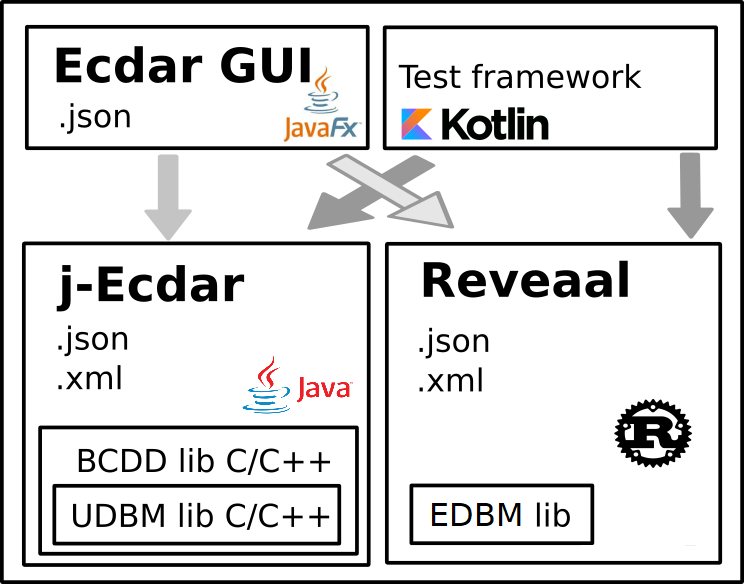
\includegraphics[width=0.75\textwidth]{common/figures/ArchOverview.png}
    \caption{The architecture of ECDAR visualized \cite{ECDARNET}.}
    \label{fig:ECDAR-architecture}
\end{figure}
%Figure old, get new

%And how they interact?

%The test framework is written in the programming language Kotlin, and ensures both the j-ECDAR and Reveaal components work correctly.
ECDAR makes use of the Kotlin test library to ensure conformance testing between j-ECDAR and Reveaal as well as automated performance testing and hand-designed test cases. 
j-ECDAR and Reveaal are engines of the tool. 
ECDAR has two engines to further ensure the correctness/reliability of the tool. 
The j-ECDAR component is an engine written in the java programming language, and its focus is readability and correctness, and ``where no effort is put into optimizing the code for speed''.\cite{ECDARNET} %TODO?:Det her er ecdar.net, ikke ecdar.net/architecture

The Reveaal engine is written in Rust and is intended to be fast and parallelizable. A goal for the Reveaal engine is to be able to run on over multiple cores on multiple machines. 

Protobuf is used to communicate between the ECDAR GUI and the two engines. In \autoref{fig:ECDAR-architecture} it can be seen as the two arrows from the GUI to the engines.

The ECDAR GUI is written with the JavaFx library, which is a Java library. 
It's a grafical user interface, which makes the tool easy to use, and sends queries to the engines through the protobuf based on the user input.

\subsection{Purpose}
ECDAR was based on the tedious process of model checking the correctness of a real-timed system, if it were to be done by hand, by using for example: Unit-testing.
Not only is it tedious when done by hand, it is also error-prone.

By providing a tool that can both be reliable and productive at testing if a new system is true to its corresponding model, we can not only ensure that time will be saved, but also the correctness of the system.
ECDAR therefore tests the correctness of the model using timed I/O automata, without involving the hand written process.
%% It parallelizes test-case generation and test execution to provide this significant speed-up.

To sum up, what the purpose of ECDAR is:
"...Ecdar that integrates conformance testing into a new IDE that now features
modelling, verification, and testing. The new tool uses model-based mutation testing, requiring only
the model and the system under test, to locate faults and to prove the absence of certain types of
faults." \cite{Gundersen_2018}



\subsection{Technologies} % Which technologies is relevant to describe in the common section?
ECDAR uses gRPC (\textbf{G}oogle \textbf{R}emote \textbf{P}rocedure \textbf{C}all) with Protocal Buffers as its remote procedure call framework.
This framework makes it possible for ECDAR to be run on a server. 
gRPC has the advantage of being able to run in any environment.


\begin{itemize}
    \item TIOA
    \item TIOTS
    \item gRPC
\end{itemize}












